  \documentclass[12pt,dvipsnames]{article}
\setcounter{section}{0}

\usepackage{amsmath,amsthm,amssymb,amsbsy}
\usepackage[spanish,es-tabla]{babel}
\decimalpoint
\usepackage{braket}
\usepackage{color}
\usepackage{enumitem}
\usepackage{fancyhdr}
\usepackage{float}
\usepackage[T1]{fontenc}
\usepackage[margin=1.5cm]{geometry} 
\usepackage{graphicx}
\graphicspath{ {images/} }
\usepackage{hyperref}
\usepackage[utf8]{inputenc}
\usepackage{listings}
\usepackage{lmodern}
\usepackage{multicol}
\usepackage{multirow}
\usepackage{pgfplots}
\usepackage{tabularx}
\usepackage{tcolorbox}
\tcbuselibrary{listings,breakable}
\usepackage{tikz}
\usetikzlibrary{babel}
\usepackage{url}
\usepackage{wrapfig}
\usepackage{xcolor}

\setlength{\parindent}{1em}
\setlength{\parskip}{1em}

\definecolor{NARANJA}{rgb}{1,0.467,0}
\definecolor{VERDE}{rgb}{0.31,1,0}
\definecolor{AZUL}{rgb}{0,0.53,1}
\definecolor{ROJO}{rgb}{1,0,0}

\hypersetup{
    colorlinks=true,
    linkcolor=ROJO,
    filecolor=magenta,      
    urlcolor=AZUL,
}
 
\pgfplotsset{compat=1.15}
 
 \renewcommand{\figurename}{Figura}

\renewcommand{\indexname}{Índice}
\renewcommand{\appendixname}{Apéndice}
\renewcommand{\contentsname}{Contenidos}
\renewcommand{\proofname}{Dem.}
\renewcommand{\tablename}{Tabla.}
\renewcommand\qedsymbol{$\blacksquare$}
\newtheorem{teo}{Teorema}[section]
\newtheorem{cor}{Corolario}[section]
\newtheorem{lem}{Lema}[section]
\newtheorem{defi}{Definición}[section]
\newtheorem{obs}{Observación}[section]
\newtheorem{prop}{Propiedades.}[section]
\newtheorem{ejem}{\textbf{\textit{$\circ \ \text{Ejemplo}$}}}[section]
\newtheorem{axi}{Axioma}[section]

\numberwithin{equation}{section}

%%%%%%%%%%%%%%%%%%%%%%%%%%%%%%%%%%%%%%%%%%%%%%%%%%%%%cajas

\newtcolorbox{post}{colback=white,colframe=red!50!black,
	colbacktitle=red!75!black, title= Postulado.}

\newtcolorbox{enu}{colframe=white!85!black, colback=white, leftrule = 10mm, sharp corners, breakable}

\newtcolorbox{solu}{colframe=black, colback=white, leftrule = 1mm, rightrule = -1mm,toprule = -1mm, bottomrule=-1mm, sharp corners, breakable}

\newtcolorbox{corre}{colframe=red, colback=white, leftrule = 1mm, rightrule = -1mm,toprule = -1mm, bottomrule=-1mm, sharp corners, breakable}

\newtcolorbox{enun}{colframe=gray, colback=white!90!black, leftrule = 1mm, rightrule = 1mm, toprule = -1mm, bottomrule=-1mm, sharp corners, breakable}

%%%%%%%%%%%%%%%%%%%%%%%%%%%%%%%%%%%%%%%%%%%%%%%%%%%%%cajas

%%%%%%%%%%%%%%%%%%%%%%%%%%%%%%%%%%%%%%%%%%%%%%%%%%%%%demarcado de soluciones

%New colors defined below
\definecolor{codegreen}{rgb}{0,0.6,0}
\definecolor{codegray}{rgb}{0.5,0.5,0.5}
\definecolor{codepurple}{rgb}{0.58,0,0.82}
\definecolor{backcolour}{rgb}{0.95,0.95,0.92}

%Code listing style named "mystyle"
\lstdefinestyle{mystyle}{
	backgroundcolor=\color{backcolour},   commentstyle=\color{codegreen},
	keywordstyle=\color{magenta},
	numberstyle=\tiny\color{codegray},
	stringstyle=\color{codepurple},
	basicstyle=\ttfamily\footnotesize,
	breakatwhitespace=false,         
	breaklines=true,                 
	captionpos=b,                    
	keepspaces=true,                 
	numbers=left,                    
	numbersep=5pt,                  
	showspaces=false,                
	showstringspaces=false,
	showtabs=false,                  
	tabsize=2
}

%"mystyle" code listing set
\lstset{style=mystyle}

\newenvironment{sol}{\begin{figure}[H]
		\begin{tikzpicture}
		\filldraw[black] (0,0) circle (3pt);
		\draw[line width = 0.5pt] (0,0) -- (4,0) node[above right]{\textbf{Solución:}};
		\end{tikzpicture}
\end{figure}}{\begin{figure}[H]
		\begin{flushright}
			\begin{tikzpicture}
			\draw[line width = 0.5pt] (0,0)-- (4,0);
			\filldraw (4,0) circle (3pt);
			\end{tikzpicture}
\end{flushright}\end{figure}}

%%%%%%%%%%%%%%%%%%%%%%%%%%%%%%%%%%%%%%%%%%%%%%%%%%%%%demarcado de soluciones
 
\begin{document}

\title{Bases ortogonales y ortonormales \\
$(\approx 85\%)$}
\date{}
\maketitle
%\tableofcontents

\begin{obs}\label{obs:1}

Las principales ventajas de poder trabajar con bases ortogonales \textemdash y, más precisamente, ortonormales\textemdash \ en espacios vectoriales con producto escalar son dos:

\begin{enumerate}
    \item algebráicamente,  simplifican enormemente el problema de encontrar los coeficientes necesarios para expresar a un vector arbitrario como combinación lineal de la base;
    
    \item geométricamente, nos permiten descomponer a cualquier vector del espacio en componentes ``independientes'', en el sentido en que podemos reescalar cualquiera de ellas sin modificar a las demás.
\end{enumerate}
\end{obs}

\begin{obs}
Siguiendo de la observación \ref{obs:1}, las ideas principales a presentar en este video son:

\begin{enumerate}[label=(\roman*)]
    \item En un espacio vectorial, podemos fácilmente hacer operaciones entre vectores distintos expresándolos como combinacines lineales de una misma base: si conocemos los coeficientes correspondientes y utilizamos los axiomas de los espacios vectoriales, entonces simplemente tenemos que hacer operaciones entre los coeficientes (en un campo).
    
    \item Dada una base y un vector no nulo arbitrario, el problema de encontrar los coeficientes para expresar a ese vector como combinación lineal de la base no es trivial. En general, resolverse computacionalmente mediante sistemas de ecuaciones, pero su complejidad aumenta dependiendo de la dimensión del espacio y de qué tipo de vectores viven en él. Sin embargo, en espacios con producto escalar este mismo problema tiene una solución general muy sencilla  si utilizamos una base ortogonal \textemdash que, como sabemos, existe por el Teorema de Gram-Schmidt\textemdash; dicha solución general es aún más simple si utilizamos una base ortonormal. Por lo tanto, las bases ortogonales y ortonormales juegan un papel privilegiado en los espacios con producto escalar.
    
    \item La solución general nos dice en términos geométricos que el problema de encontrar los coeficientes se trivializa en espacios con producto escalar si descomponemos al vector no nulo en sus componentes a lo largo de los ejes en los que viven los vectores de la base ortogonal/ortonormal.
\end{enumerate}
\end{obs}

\newpage
\section{Primera escena (motivación y definición de base)}

Supongamos que tenemos un espacio vectorial y queremos calcular la suma entre dos vectores arbitrarios. Como sabemos, la suma vectorial es una operación binaria conmutativa, por lo que a cada par de vectores del espacio le asigna un vector del espacio. El problema al que nos enfrentamos es, ¿cómo encontramos a dicho vector? Podríamos pensar en tener un registro (e.g., una tabla) de todos los pares de vectores del espacio junto con el resultado de su suma; sin embargo, si consideramos espacios vectoriales sobre campos infinitos \textemdash como el campo real o el campo complejo\textemdash, lo anterior sólo sería factible en el caso trivial. Nuestro objetivo, entonces, es encontrar un método general para calcular la suma de dos vectores arbitrarios.

Para empezar a solucionar el problema, pensemos primero en cómo lo haríamos en los casos más sencillos: por ejemplo, si los vectores sumados fueran iguales, podríamos aplicar los axiomas de existencia de un elemento identidad del reescalamiento y de distributividad del reescalamiento con respecto a la suma escalar para ver que la suma de ellos debe ser igual al reescalamiento del vector original por dos. Más aún, si ambos vectores fueran reescalamientos de un mismo vector, podríamos aplicar el mismo axioma de distributividad para encontrar nuestro resultado. Aún más generalmente, si pudiéramos expresar a ambos vectores como combinaciones lineales de un mismo conjunto, podríamos aplicar el axioma de conmutatividad de la suma vectorial junto con los axiomas anteriores para encontrar nuestro resultado. En este último caso, incluso podríamos fácilmente calcular cualquier combinación lineal los dos vectores, aplicando axiomas de los espacios vectoriales\footnote{Mostramos una nota al pie que diga ``Ver la Pregunta al final del video.''}.

Por lo tanto, cuando trabajamos en espacios vectoriales es de gran utilidad contar con algún conjunto de vectores con el cual podamos expresar a \emph{cualquier} vector del espacio como combinación lineal de sus elementos, lo que equivale a decir que dicho conjunto genere a todo el espacio. Es más útil aún si cada uno de los cálculos realizados con el conjunto de vectores corresponde a un único vector del espacio, lo que equivale a que sea linealmente independiente, ya que esto implica que cualquier vector generado por el conjunto se expresa como una combinación lineal única de sus elementos. Son precisamente estas dos características las que definen el concepto de \emph{base} de un espacio vectorial. De la definición, podemos ver que un mismo espacio vectorial puede tener muchas bases distintas, incluso una infinidad de ellas\footnote{Mostramos una nota al pie que diga ``Ver los Ejercicios 3.1 y 3.2 al final del video.''}; sin embargo, se puede demostrar que todas tienen la misma cardinalidad, a la cual se le conoce como la \emph{dimensión} del espacio. \\

\newpage
\section{Segunda escena (utilidad de bases ortogonales y ortonormales)}

Hasta ahora, hemos visto que si tenemos un espacio vectorial y una base para él entonces cualquier vector del espacio puede ser expresado de manera única como combinación lineal de la base, y esto es de gran utilidad para hacer cálculos con vectores; sin embargo, nuestro método aún está incompleto, pues no hemos considerado la siguiente pregunta: dado un espacio vectorial de dimensión finita, un vector no nulo cualquiera y una base arbitraria del espacio, ¿cómo encontramos los coeficientes necesarios para expresar a nuestro vector como combinación lineal de dicha base?

\begin{align*}
    & & &\text{dim}(V)=k<\infty& & &\\
    \\
    \beta&=\{\vec{b}_1,...,\vec{b}_k\} \ \ \text{base de} \ \ V& & & & &\\
    \\
    \langle\beta&\rangle = V, \ \ \beta \ \ \text{es} \ \ l.i.& & & & & \\
    \\
    \vec{v}&= c_1\vec{b}_1 + ... + c_k\vec{b}_k& & & & & \\
    \\
    \\
    \\
    & \quad \quad \ \ \text{¿}c_1,...,c_k\text{?} & & & & &
\end{align*}

Veamos cómo podríamos representar este problema en el caso del plano real. Tenemos a nuestro vector no nulo cualquiera y nuestra base arbitraria. Como la base genera a todo el espacio y es linealmente independiente, sabemos que existe una combinación lineal única de sus elementos que da como resultado a nuestro vector. Sin embargo, no sabemos cómo encontrar a los coeficientes de dicha combinación lineal. Este es el problema que queremos resolver. Vamos primero a resolverlo de manera general, y luego volveremos al caso del plano real para representar su solución.

Regresando al planteamiento general, este problema puede llegar a ser muy complicado, ya que nuestros vectores podrían ser funciones, n-tuplas, matrices, etc. y tendríamos que resolver un sistema de ecuaciones -mediante el método computacional de nuestra preferencia-, el cual aumentaría en complejidad a medida que aumente la dimensión de nuestro espacio. Sin embargo, se puede resolver de forma sencilla en espacios vectoriales con producto escalar si utilizamos bases ortogonales y ortonormales.

Antes de ver cómo se resuelve el problema para estos casos, observemos lo siguiente. Si tenemos un espacio vectorial de dimensión finita con producto escalar, entonces podemos aplicarle el Proceso de Gram-Schmidt a cualquier base del espacio para obtener un conjunto ortogonal que genera a todo el espacio y que es linealmente independiente, como vimos en el video anterior. Es decir, podemos obtener una \emph{base ortogonal} para nuestro espacio a partir de cualquier base arbitraria. Análogamente, si a cualquier base le aplicamos el Proceso de Gram-Schmidt modificado, obtenemos una \emph{base ortonormal} de nuestro espacio. Este resultado se conoce como el Teorema de Gram-Schmidt.

Ahora, supongamos que $\Gamma$ es una base ortogonal de $V$. Entonces, nuevamente, sabemos que existen coeficientes tales que la siguiente ecuación se cumple. ¿Pero cómo encontramos a estos coeficientes?

\begin{align*}
    \beta&=\{\vec{b}_1,...,\vec{b}_k\} \ \ \text{base de} \ \ V& &\Gamma=\{\vec{g}_1,...,\vec{g}_k\} \ \ \text{base ortogonal de} \ \ V& & &\\
    \\
    \langle\beta&\rangle = V, \ \ \beta \ \ \text{es} \ \ l.i.& &\langle\Gamma\rangle = V, \ \ \langle \vec{g}_j , \vec{g}_i \rangle = \begin{cases} \langle\vec{g_i}, \vec{g}_i\rangle \ \ \text{si} \ \ j = i \\ \quad 0 \quad \ \ \ \text{si} \ \ j\neq i \end{cases}& & &\\
    \\
    \vec{v}&= c_1\vec{b}_1 + ... + c_k\vec{b}_k& &\quad \quad \quad \quad \vec{v}= d_1\vec{g}_1 + ... + d_k\vec{g}_k& & & \\
    \\
    \\
    &\quad \quad \quad \quad \text{¿}c_i\text{?}& & \quad \quad \quad \quad \quad \quad \quad \quad \text{¿}d_i\text{?} & & &
\end{align*}

Observemos lo siguiente: si tomamos al $i$-ésimo elemento de la base ortogonal, aplicamos el producto escalar con ese elemento a ambos lados de la ecuación, luego, hacemos uso de las propiedades lineales del producto escalar en la primera entrada y, finalmente, utilizamos el hecho de que nuestra base es ortogonal, podemos encontrar una expresión sumamente sencilla para el $i$-ésimo coeficiente: simplemente se obtiene a través de dos productos escalares y una división.

\begin{align*}
    & & & \quad \quad \vec{v}= d_1\vec{g}_1 + ... + d_k\vec{g}_k& & & \\
    \cline{1-8}
    & & &\langle \vec{v} , \vec{g}_i \rangle = \langle d_1\vec{g}_1 + ... + d_k\vec{g}_k , \vec{g_i} \rangle& & & \\
    \cline{1-8}
    & & &\langle \vec{v} , \vec{g}_i \rangle = \langle d_1\vec{g}_1,\vec{g}_i\rangle + ... + \langle d_k\vec{g}_k , \vec{g_i} \rangle& & & \\
    \cline{1-8}
    & & &\langle \vec{v} , \vec{g}_i \rangle = d_1\langle \vec{g}_1, \vec{g}_i\rangle + ... + d_k\langle \vec{g}_k , \vec{g_i} \rangle& & & \\
    \cline{1-8}
    & & &\langle \vec{v} , \vec{g}_i \rangle = \sum_{j=1}^k d_j\langle \vec{g}_j, \vec{g}_i\rangle& & & \\
    \cline{1-8}
    & & &\langle \vec{v} , \vec{g}_i \rangle = d_i \langle\vec{g}_i, \vec{g}_i\rangle& & & \\
    \cline{1-8}
    & & &\frac{\langle \vec{v} ,\vec{g}_i \rangle}{\langle\vec{g}_i, \vec{g}_i\rangle} = d_i& & &
\end{align*}

Como esto es válido para toda $i$, tenemos el siguiente resultado para cualquier vector arbitrario de nuestro espacio con producto escalar:

\[d_i = \frac{\langle \vec{v} ,\vec{g}_i \rangle}{\langle\vec{g}_i, \vec{g}_i\rangle} \quad \forall i\in\{1,...,k\} \]

\begin{align*}
    \beta&=\{\vec{b}_1,...,\vec{b}_k\} \ \ \text{base}& &\Gamma=\{\vec{g}_1,...,\vec{g}_k\} \ \ \text{base ortogonal}& & &\\
    \\
    \langle\beta&\rangle = V, \ \ \beta \ \ \text{es} \ \ l.i.& &\langle\Gamma\rangle = V, \ \ \langle \vec{g}_j , \vec{g}_i \rangle = \begin{cases} \langle\vec{g_i}, \vec{g}_i\rangle \ \ \text{si} \ \ j = i \\ \quad 0 \quad \ \ \ \text{si} \ \ j\neq i \end{cases}& & &\\
    \\
    \vec{v}&= c_1\vec{b}_1 + ... + c_k\vec{b}_k& &\quad \quad \quad \quad \vec{v}= d_1\vec{g}_1 + ... + d_k\vec{g}_k& & & \\
    \\
    \\
    &\quad \quad \quad \quad \text{¿}c_i\text{?}& &\quad \quad \quad \quad \quad \quad d_i = \frac{\langle \vec{v} ,\vec{g}_i \rangle}{\langle\vec{g}_i, \vec{g}_i\rangle}& & &
\end{align*}

Más aún, haciendo un procedimiento análogo con una base ortonormal $N$ de $V$, obtenemos que el cálculo de los coeficientes buscados se efectúa simplemente a través de un producto escalar.

\begin{align*}
    \beta&=\{\vec{b}_1,...,\vec{b}_k\} \ \ \text{base}& &\Gamma=\{\vec{g}_1,...,\vec{g}_k\} \ \ \text{base \emph{ortogonal}}& &N=\{\hat{n}_1,...,\hat{n}_k\} \ \ \text{base \emph{ortonormal}}&\\
    \\
    \langle\beta&\rangle = V, \ \ \beta \ \ \text{es} \ \ l.i.& &\langle\Gamma\rangle = V, \ \ \langle \vec{g}_j , \vec{g}_i \rangle = \begin{cases} \langle\vec{g_i}, \vec{g}_i\rangle \ \ \text{si} \ \ j = i \\ \quad 0 \quad \ \ \ \text{si} \ \ j\neq i \end{cases}& &\langle N \rangle = V, \ \ \langle \vec{n}_j , \vec{n}_i \rangle = \delta_{ij}&\\
    \\
    \vec{v}&= c_1\vec{b}_1 + ... + c_k\vec{b}_k& &\quad \quad \quad \quad \vec{v}= d_1\vec{g}_1 + ... + d_k\vec{g}_k& &\quad \quad \quad \quad \vec{v}= e_1\hat{n}_1 + ... + e_k\hat{n}_k& \\
    \\
    \\
    &\quad \quad \quad \quad \text{¿}c_i\text{?}& &\quad \quad \quad \quad \quad \quad d_i = \frac{\langle \vec{v} ,\vec{g}_i \rangle}{\langle\vec{g}_i, \vec{g}_i\rangle}& &\quad \quad \quad \quad \quad \quad e_i = \langle \vec{v} ,\hat{n}_i \rangle& \\
    \\
    \cline{1-8}
    &\Gamma=\{\vec{g}_1,...,\vec{g}_k\} \ \ \text{base ortogonal}& & & &N=\{\hat{n}_1,...,\hat{n}_k\} \ \ \text{base \emph{ortonormal}}&\\
    \\
    \\
    \\
    &\quad \quad \quad \quad \vec{v}= \sum_{i=1}^k \frac{\langle \vec{v} ,\vec{g}_i \rangle}{\langle\vec{g}_i, \vec{g}_i\rangle}\vec{g}_i& & & &\quad \quad \quad \quad \vec{v}= \sum_{i=1}^k \langle \vec{v} ,\hat{n}_i \rangle \hat{n}_i
\end{align*}

Dada su utilidad, durante el resto de la serie de videos utilizaremos bases ortonormales.

\newpage
\section{Tercera escena}
Regresemos ahora a la representación geométrica del problema en el caso del plano real. Vamos a empezar a resolver el problema simplificándolo un poco, convirtiéndolo en un caso particular más sencillo de resolver, y viendo si esa solución nos ayuda a resolver el caso más general.

Supongamos que nuestro vector no nulo vive en el mismo eje que uno de los elementos de la base. En ese caso, como dicho elemento de la base genera a todos los vectores del mismo eje porque el espacio es real, entonces existe un escalar por el cual podemos multiplicar a ese elemento de la base para obtener a nuestro vector no nulo.

¿Cómo lo encontramos? Aprovechando el hecho de que nuestro espacio tiene producto escalar. Recordemos que mediante el producto escalar podemos encontrar la proyección vectorial de nuestro vector sobre el elemento de la base. Esto nos da como resultado la componente de nuestro vector que vive en el subespacio generado por el elemento de la base... pero, en este caso, ¡esa componente coincide con todo el vector! Manipulando un poco la expresión de la proyección vectorial, encontramos el escalar por el cual debemos multiplicar al elemento de la base para obtener a nuestro vector. Esto implica que el segundo coeficiente es igual a cero. Así, hemos encontrado nuestra solución.

\begin{figure}[h!]
    \centering
    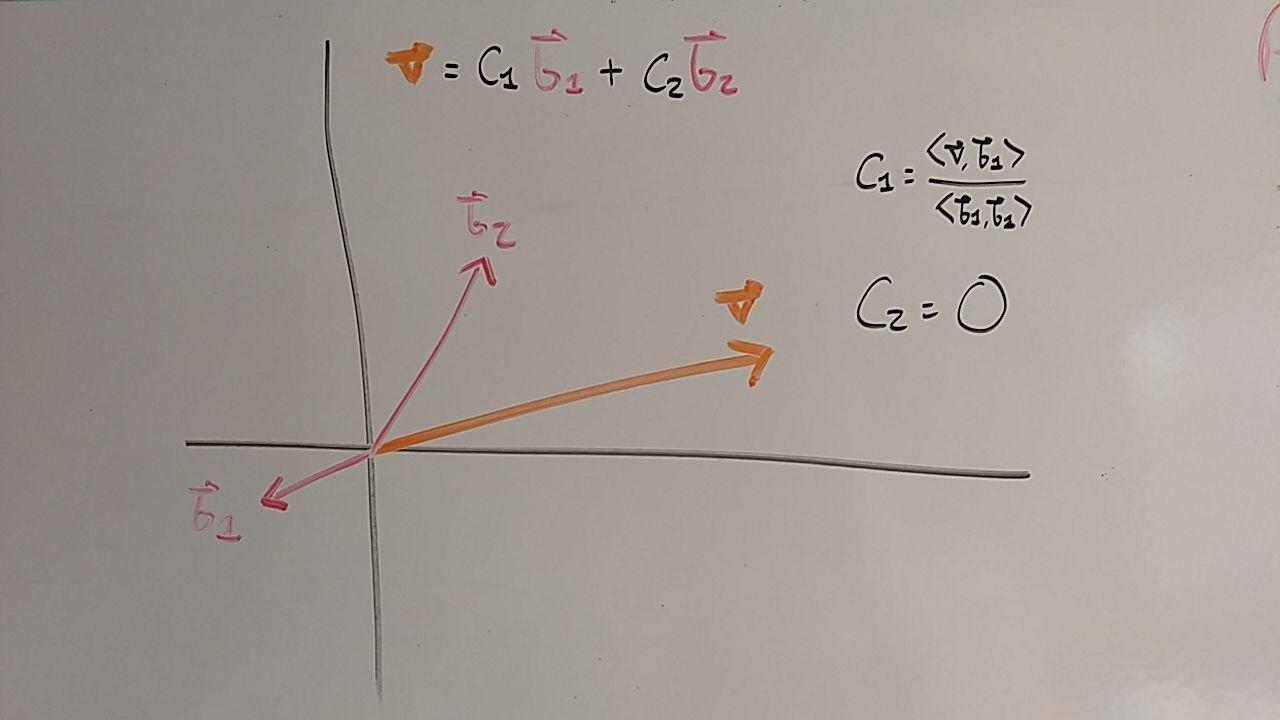
\includegraphics[width=\textwidth]{3/Bases_ortogonales_y_ortonormales_3-1.jpg}
\end{figure}

\newpage
Como queremos los coeficientes para cualquier vector no nulo del espacio, intentemos aplicar este método de proyecciones vectoriales para un vector no nulo que no vive en el mismo eje que alguno de los elementos de la base. Observemos que en este caso la combinación lineal obtenida no coincide con nuestro vector, pues existe un cierto sobrelape entre las dos proyecciones vectoriales.

\begin{figure}[h!]
    \centering
    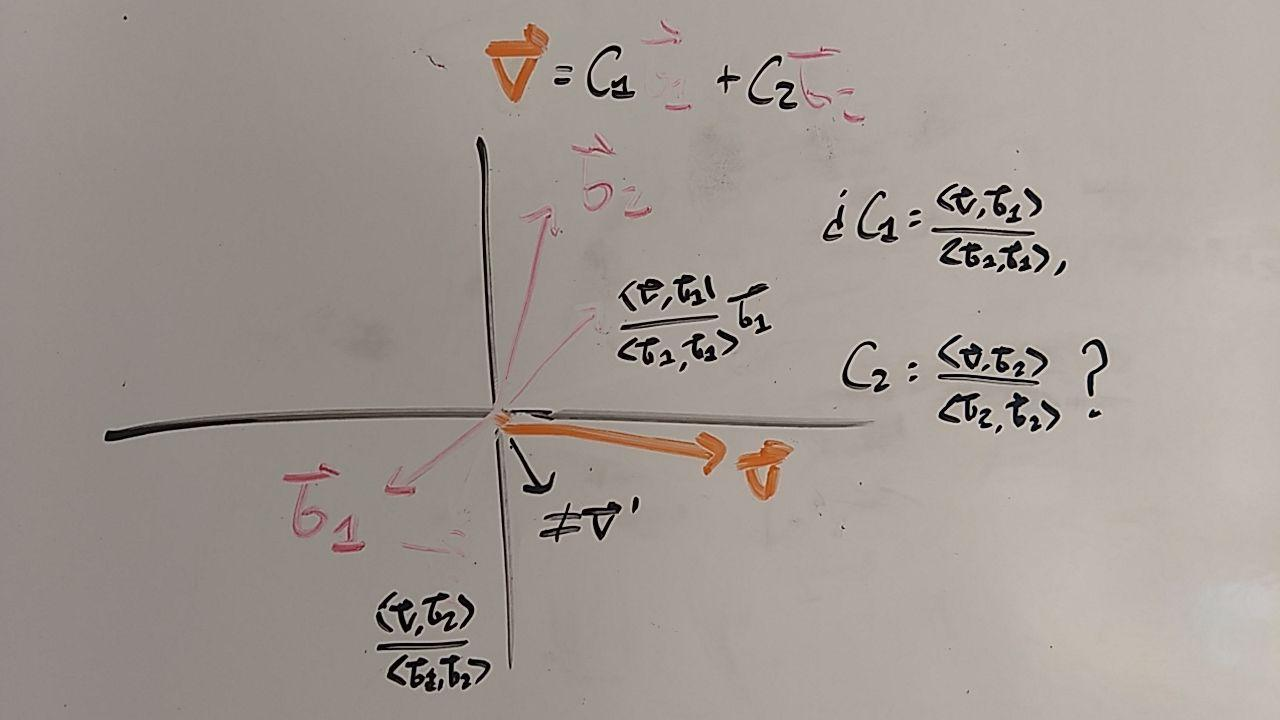
\includegraphics[width=16cm]{3/Bases_ortogonales_y_ortonormales_3-2.jpg}
\end{figure}

Esto es debido a que los vectores sobre los que estamos proyectando \emph{no son ortogonales}, por lo que cualquier proyección vectorial sobre uno de ellos carga una componente a lo largo del eje del otro vector. 

\begin{figure}[h!]
    \centering
    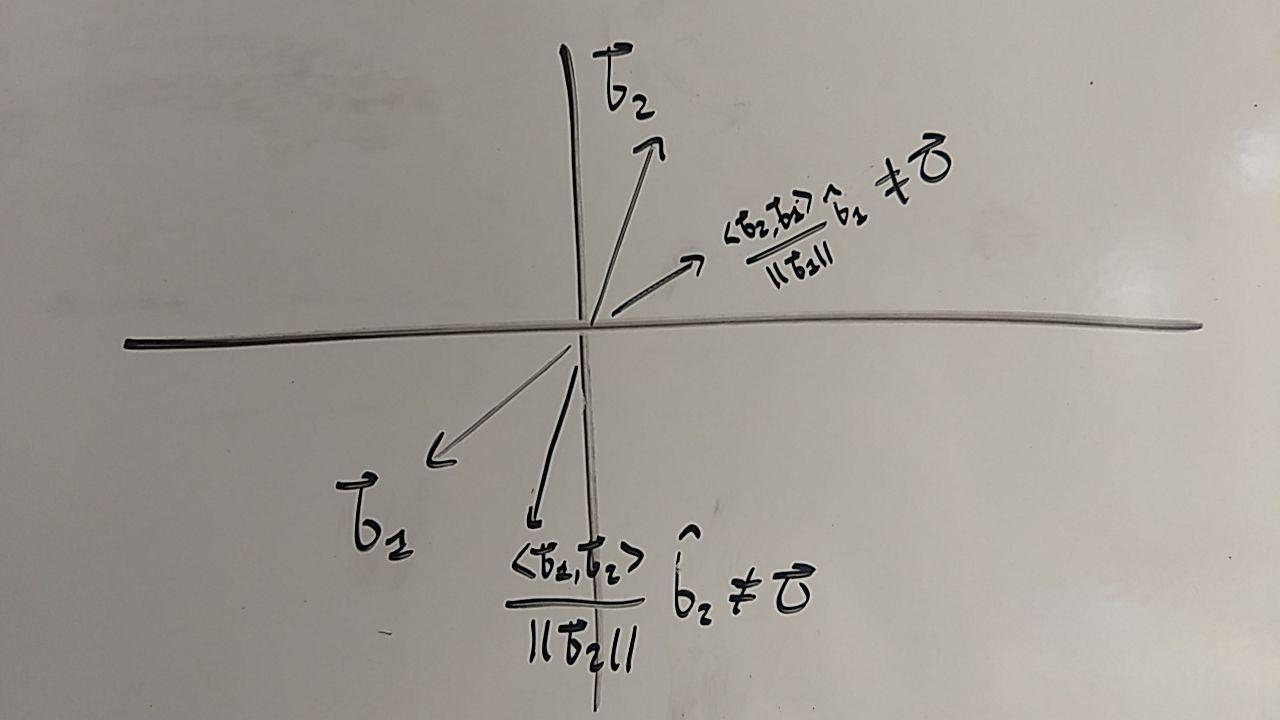
\includegraphics[width=16cm]{3/Bases_ortogonales_y_ortonormales_3-3.jpg}
\end{figure}

\newpage
Ahora, si ortogonalizamos esta base mediante el Proceso de Gram-Schmidt, eliminamos el problema anterior, y obtenemos una solución válida para cualquier vector no nulo del espacio.

\begin{figure}[h!]
    \centering
    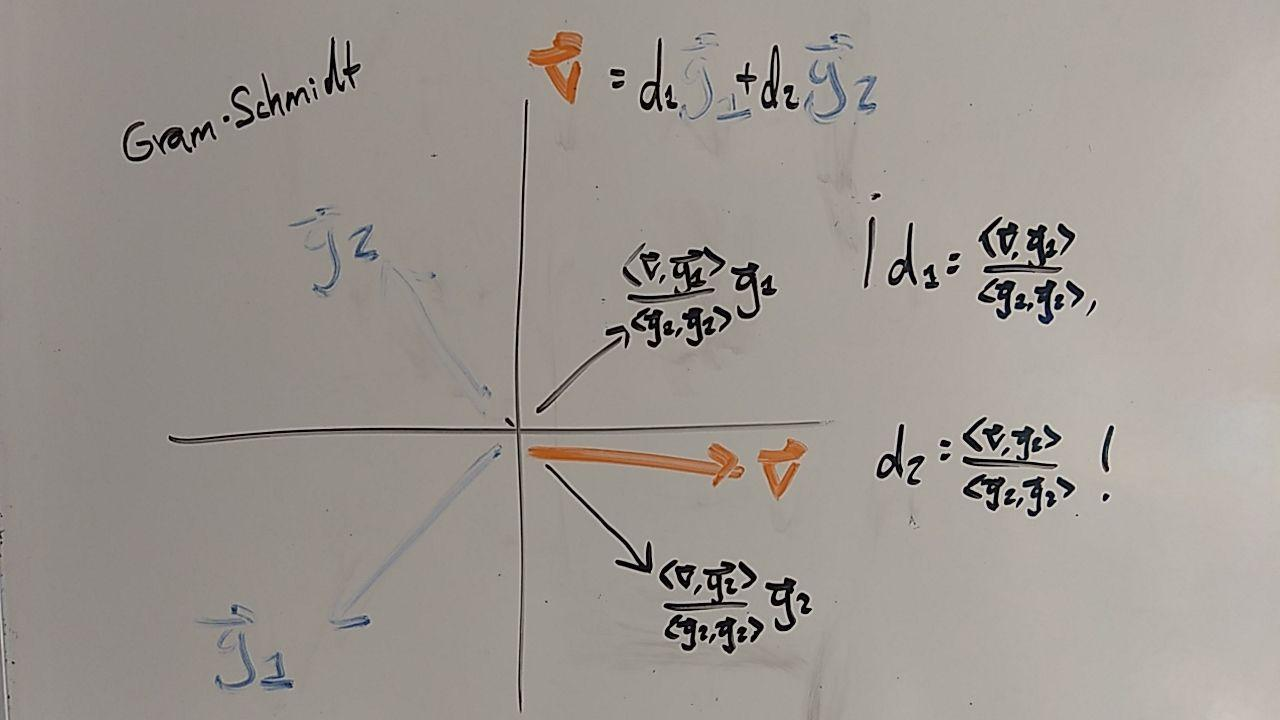
\includegraphics[width=16cm]{3/Bases_ortogonales_y_ortonormales_3-4.jpg}
\end{figure}

Si en vez de ortogonalizar la base original la ortonormalizamos meidante el Proceso de Gram-Schmidt modificado, obtenemos una solución aún más sencilla. Esta es la interpretación geométrica de la solución general que habíamos encontrado algebráicamente.

\begin{figure}[h!]
    \centering
    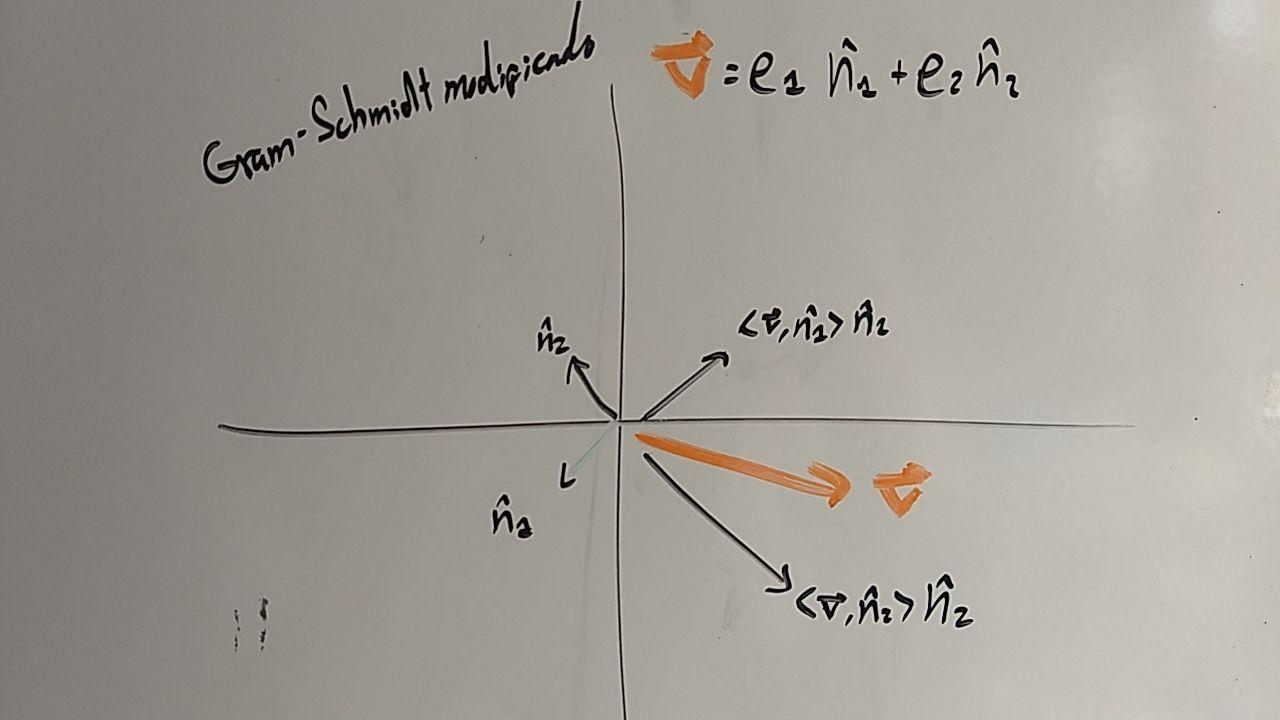
\includegraphics[width=16cm]{3/Bases_ortogonales_y_ortonormales_3-5.jpg}
\end{figure}

Esta es precisamente la intuición geométrica detrás de las soluciones algebráicas que obtuvimos anteriormente. Esta misma intuición puede ser extendida a cualquier espacio vectorial de dimensión finita, siempre y cuando tenga un producto escalar, para facilitar las operaciones entre vectores del espacio, aprovechando así las ventajas que ofrecen las bases ortogonales y ortonormales\footnote{Quizá mostrar en pantalla una nota sobre bases ortogonales y ortonormales en espacios de dimensión finita, y poner algo en las referencias.}.

\newpage
\section{Escena final}

Ejercicio 3.1 Sea $(V,K)$ un espacio vectorial de dimensión finita con base $\{\vec{b}_1,...,\vec{b}_k\}$. Demuestra que $$\{c_1\vec{b}_1,...,c_k\vec{b}_k\}$$ es una base de $(V,K)$ para $c_1,...,c_k\in K$ no nulos. Concluye que cualquier espacio vectorial sobre un campo infinito tiene una infinidad de bases. \\

Ejercicio 3.2 Demuestra que cualesquiera dos bases de un mismo espacio vectorial deben tener la misma cardinalidad. \\

Pregunta Tener una base para un espacio vectorial es útil para calcular la suma de dos vectores arbitrarios de ese espacio, pero también sirve para calcular cualquier combinación lineal de dos vectores arbitrarios. ¿Qué axiomas de los espacios vectoriales aplicarías en este caso, y cómo podrías generalizarlo?

\end{document}